\begin{surferPage}[Octique de Chmutov]{Une Octique de Chmutov}
    Une propriété de l'octique de Chmutov $\text{Chm}_{d}, \ d=8$ attire l'attention,
    sa symétrie.
    Elle peut être retrouvée en observant l'équation :
    \[\text{Chm}_{d}\colon T_d(x) + T_d(y) + T_d(z) + 1 = 0,\]
     où $T_d$ désigne le polynôme de Tchebychev (image de gauche).
    La courbe $T_8(x)+T_8(y)=0$ est représentée à droite :
    
     \begin{center}
      \begin{tabular}{c@{\quad}c}
        \begin{tabular}{c}
          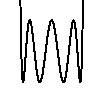
\includegraphics[height=1.75cm]{./../../common/images/Tcheb_008.pdf}
        \end{tabular}    
        &
        \begin{tabular}{c}
          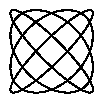
\includegraphics[height=1.75cm]{./../../common/images/Tcheb_2d_008.pdf}
        \end{tabular}    
      \end{tabular}
    \end{center}
    \vspace{-0.3cm}
    Le passage entre ces images et celle, interactive, de la forme
    de la surface est assez direct.


Ces équations ont été données par S.V.\ Chmutov au début des années 1980.
    Elles établissaient à l'époque le record pour la plupart des valeurs de $d$
    du nombre maximal $\mu(d)$ de singularités pour les surfaces de degré $d$. 
    Dans les années 1990, Chmutov améliora son propre record, puis en 2005, S.~Breske,
    O.~Labs et D.~van~Straten adaptèrent cette construction pour fournir des surfaces réelles
    avec toutes leurs singularités réelles.
\end{surferPage}